\section{提示词}\label{app:prompt}

\paragraph{声明分解与双立场论证（中文）}
下面是 \method{} 结构化调用的系统提示与用户提示。$a^+$ 与 $a^-$ 的书写顺序按样本编号的奇偶交替，这里给出先写支持论证的版本。输出受 JSON schema 约束，字段依次为 \texttt{first\_impression}、\texttt{claims}（每条含 \texttt{claim}、\texttt{type}、\texttt{sent}、两条论证与 \texttt{suspicion}）和 \texttt{overall}。

{\small\setlength{\parindent}{0pt}\begin{quote}
你是一名严谨的事实核查分析员。你无法联网检索，只能依据消息文本本身以及你已有的常识和背景知识进行分析。\par
\vspace{3pt}
下面是一条已按句编号的新闻或社交媒体消息。请对它做“声明分解 + 正反论证”分析，只输出一个 JSON 对象。\par
\vspace{3pt}
【步骤】\par
0. 先不做分析，凭第一印象填写 first\_impression：整条消息是虚假或误导性信息的可能性，1=几乎肯定属实，2=较可能属实，3=无法判断，4=较可能不实，5=几乎肯定不实。\par
1. 找出消息中最核心、可被核查的原子声明（claim），按重要性排序，共 1–6 条，尽量覆盖消息中彼此不同的事实陈述。\par
\hspace*{3em}- 一条声明只陈述一件事，并且要自包含：补全主语、时间、地点，不要出现“他”“该公司”“此事”等指代。\par
\hspace*{3em}- 保留归属：原文若是“某人/某机构称……”，声明里必须保留“某人称”，不要改写成既成事实。\par
\hspace*{3em}- 不要抽取情绪宣泄、呼吁转发、提问、投票等非事实内容。\par
2. 对每条声明写出两条有针对性的理由，各不超过 60 字：\par
\hspace*{3em}- support：认为这条声明可信的最强理由；\par
\hspace*{3em}- refute：认为这条声明可疑的最强理由。\par
\hspace*{3em}理由要结合常识、背景知识、逻辑和文本内部的一致性，针对这条声明本身来写，避免“细节具体”“缺乏来源”这类对任何消息都适用的套话；不要写“所以这是真/假新闻”之类的结论。\par
3. 写完两条理由后，权衡哪一方更站得住脚，再给出 suspicion（该声明不属实的可能性）：\par
\hspace*{3em}1–5，含义同第 0 步。\par
4. type：fact=事件或事实陈述，number=数字或统计，quote=引述他人说法，opinion=预测、评价或观点。\par
5. sent：这条声明主要出自哪一句（填句子编号）。\par
6. 最后填写 overall（整体判断）：综合上面各条声明的分析，并考虑标题与正文是否一致、信息来源是否明确可靠、是否煽动情绪或夸大其词、叙述是否自洽，对整条消息做出评估。同样先写 support（认为整条消息可信的最强理由）和 refute（认为整条消息不可信的最强理由），再给出 suspicion（整条消息是虚假或误导性信息的可能性，1–5，含义同上）。\par
\vspace{3pt}
【消息】\par
〈按句编号的消息文本：[1] …… [2] ……〉\par
\end{quote}}


\paragraph{声明分解与双立场论证（英文）}

{\small\setlength{\parindent}{0pt}\begin{quote}
You are a rigorous fact-checking analyst. You cannot search the web; rely only on the message itself and on your own commonsense and background knowledge.\par
\vspace{3pt}
Below is a news article or social media message whose sentences have been numbered. Perform a "claim decomposition + two-sided argumentation" analysis and output a single JSON object only.\par
\vspace{3pt}
Steps:\par
0. Before any analysis, fill in first\_impression from your first impression: how likely the whole message is false or misleading, 1 = almost certainly true, 2 = more likely true, 3 = cannot tell, 4 = more likely untrue, 5 = almost certainly untrue.\par
1. Extract the most central, checkable atomic claims of the message, ordered by importance: between 1 and 6 claims, covering the distinct factual assertions of the message.\par
\hspace*{3em}- Each claim states exactly one thing and must be self-contained: fill in the subject, time and place; do not use pronouns or references such as "he", "the company", "this".\par
\hspace*{3em}- Keep the attribution: if the text says "X said/claimed ...", the claim must keep "X said"; do not rewrite it as an established fact.\par
\hspace*{3em}- Do not extract emotional venting, calls to share, questions, or other non-factual content.\par
2. For each claim write two targeted arguments, each at most 40 words:\par
\hspace*{3em}- support: the strongest argument that this claim is credible;\par
\hspace*{3em}- refute: the strongest argument that this claim is doubtful.\par
\hspace*{3em}Ground the arguments in commonsense, background knowledge, logic and the internal consistency of the text, and make them specific to this claim; avoid boilerplate that would fit any message (e.g. "it gives specific details", "no source is given"). Do not state a verdict such as "so this news is real/fake".\par
3. Only after writing both arguments, weigh which side is stronger and give suspicion (how likely the claim is NOT true):\par
\hspace*{3em}1-5, same scale as in step 0.\par
4. type: fact = an event or factual statement, number = a figure or statistic, quote = a reported statement of someone, opinion = a prediction, evaluation or opinion.\par
5. sent: the number of the sentence this claim mainly comes from.\par
6. Finally fill in overall (overall judgement): combine your analysis of the claims above with whether headline and body agree, whether sources are explicit and reliable, whether the message is sensational or exaggerated, and whether the narrative is self-consistent, and assess the message as a whole. Again write support (the strongest argument that the message is credible) and refute (the strongest argument that the message is not credible) first, then give suspicion (how likely the whole message is false or misleading, 1-5, same scale as above).\par
\vspace{3pt}
Message:\par
\textless{}the message with numbered sentences: [1] ... [2] ...\textgreater{}\par
\end{quote}}


\paragraph{基线的提示词}
零样本、零样本 CoT 以及 ARG 的两个视角（文字描述、常识）使用 ARG 论文附录中的提示\citep{hu2024bad}；FactGuard 的 topic-content 抽取使用其官方仓库中的提示\citep{he2026factguard}。为便于从输出中解析判断，我们在 ARG 的提示后追加了一句长度与输出格式的要求。

\paragraph{风格改写（中文）}

{\small\setlength{\parindent}{0pt}\begin{quote}
你是一名资深编辑。\par
\vspace{3pt}
请把下面这条消息改写成〈目标文风：官方媒体通稿（如新华社、人民日报官方微博）那种客观、严谨、克制的；或：自媒体营销号、标题党那种夸张、煽情、口语化的〉文风。\par
要求：\par
1. 保留原文的全部事实信息（人物、机构、时间、地点、数字、事件、引述内容），不得增加、删除或修改任何事实；\par
2. 只改变措辞、语气和表达方式；\par
3. 篇幅与原文相近；\par
4. 只输出改写后的文本，不要任何解释。\par
\vspace{3pt}
原文：\par
〈原文〉\par
\end{quote}}


\paragraph{单句事实篡改（中文）}

{\small\setlength{\parindent}{0pt}\begin{quote}
你是一名事实核查研究助手，正在为虚假信息检测模型构造受控的测试样本。\par
\vspace{3pt}
下面给出一条消息以及其中的一句话。请对这句话做一处最小的事实性改动，使它陈述的事实与原文不同。\par
做法：从这句话里选一个尽量短的连续片段 original\_span（必须与句中文字完全一致），给出替换它的文字 new\_span；除这个片段外，句子的其余部分保持不变。\par
change\_type 说明改动类型：negation=肯定与否定互换，number=修改数字或数量，time=修改时间或日期，entity=替换人物、机构、地点或事物，outcome=颠倒结果、因果或程度。\par
要求：\par
1. 替换后的句子通顺自然；\par
2. 改动必须改变句子陈述的事实，不能是同义改写、补全残缺文字或修正错别字；\par
3. 不要加入“据说”“可能”之类的模糊词，不要改动标点。\par
只输出一个 JSON 对象。\par
\vspace{3pt}
消息全文：\par
〈消息全文〉\par
\vspace{3pt}
需要改动的句子：\par
〈被选中的句子〉\par
\end{quote}}


\section{实现细节}\label{app:impl}

\paragraph{离线生成}
LLM 输出用 vLLM\citep{kwon2023vllm} 批量生成。分析类提示（声明分解、零样本、CoT、ARG 的两个视角）采用贪心解码；topic-content 抽取沿用 FactGuard 仓库的温度 0.2；风格改写与事实篡改由 Qwen3-8B 在关闭思考模式、温度 0.3 下生成。声明分解的最大输出长度为 1{,}200 个 token，输出无法解析时以更宽松的约束重试一次。两个数据集共 15{,}522 条新闻，首次生成即可解析的比例为 \ptwo{CN/cost/clara_first_attempt_rate}\%（中文）与 \ptwo{EN/cost/clara_first_attempt_rate}\%（英文），其余在重试后全部解析成功。

\paragraph{裁决器}
隐藏层维度 384，dropout 0.2；新闻、声明、声明--论证对的最大长度分别为 170、48 与 128 个 token。优化器为 Adam（FactGuard 按其官方实现用 AdamW），权重衰减 $5\times10^{-5}$。标量参数（$\alpha,\alpha_0,\gamma,b$ 以及 BERT+ZS 的融合权重 $w$）单独使用学习率 $10^{-2}$：在编码器的学习率下，Adam 在整个训练过程中至多把一个标量移动约 0.02，这类参数实际上不会离开初始值。可训练的编码器层用混合精度计算。

\paragraph{LoRA-LLM}
秩 16，缩放系数 32，dropout 0.05，作用于注意力与前馈层的全部线性投影；学习率 $10^{-4}$，线性预热 6\% 后线性衰减，等效批大小 16，训练 3 轮，每轮结束后在验证集上评估并按 macro-F1 选择。

\paragraph{蒸馏}
ARG-D 与 FactGuard-D 的蒸馏权重与学习率取自各自的官方脚本。\student{} 的三个蒸馏权重均为 1，学习率与教师相同。

\paragraph{软硬件}
全部实验在单张 RTX 3090（24\,GB）上完成。生成环境为 vLLM 0.26 与 PyTorch 2.11，训练环境为 PyTorch 2.4、Transformers 4.46 与 PEFT 0.13。

\paragraph{与官方设置的差异}
（1）LLM 输出。ARG 官方使用 GPT-3.5 的理由。FactGuard 官方用本地部署的 DeepSeek-R1-Distill-Llama-8B（中文）与 SOLAR-10.7B（英文）抽取 topic-content，要求抽取结果与原文的余弦相似度超过阈值，否则重新抽取；其常识理由沿用 ARG 数据中的 GPT-3.5 理由\citep{he2026factguard}。本文把所有 LLM 输出统一为 Qwen2.5-7B；topic-content 用其官方仓库中的提示一次生成，没有做相似度过滤与重试，这可能对 FactGuard 不利。（2）编码器。FactGuard 官方在中文上使用 bert-base-chinese、英文上使用 RoBERTa，本文为所有方法统一了编码器。（3）FactGuard 的损失。可用性损失以 LLM 判断 $y_{\mathrm{llm}}$ 为目标；当 LLM 未给出明确判断时，本文取目标为 0.5。文本损失中 topic-content 分支的目标按论文公式取标签 $y$。前向计算与官方代码一致，包括其中以 topic-content 代替新闻原文参与交叉注意力的做法。（4）官方脚本只给出单个随机种子的配置，本文为多种子均值。（5）训练时冻结层的输出取自缓存，可训练层使用混合精度（附录~\ref{app:live}）。因此本文复现的数值与原论文不可直接比较，原论文报告的数值见 \ref{sec:main-results} 节。

\section{冻结层缓存的核对}\label{app:live}

表~\ref{tab:live} 比较了“缓存冻结层输出”与“每步重新计算冻结层（不缓存、不使用混合精度）”两种训练方式，后者与官方实现的计算完全一致。

\begin{table}[H]
\centering\small
\caption{缓存与每步重算的对比（Weibo21，3 个种子）。时间为单次运行（含评测）的平均秒数。}\label{tab:live}
\fittable{tables/live.tex}
\end{table}

\section{学习率网格的全部结果}

\begin{table}[H]
\centering\small
\caption{各方法在两个学习率下的验证集与测试集 macro-F1（5 个种子）。加粗的验证集数值对应被选中的配置。}\label{tab:grid}
\fittable{tables/grid.tex}
\end{table}

\section{显著性检验}

\begin{table}[H]
\centering\small
\caption{\method{} 与各方法在测试集 macro-F1 上的差异（\method{} 减去对方）。置信区间与 $p$ 值来自对测试样本的配对 bootstrap。}\label{tab:sig}
\fittable{tables/sig.tex}
\end{table}

\section{敏感性分析}\label{app:sens}

\method{} 的损失权重与错配负例比例是预先设定的。图~\ref{fig:sens} 给出每个超参数另取两个值时的结果，以及声明数上限 $K$ 的影响。

\begin{figure}[H]
\centering
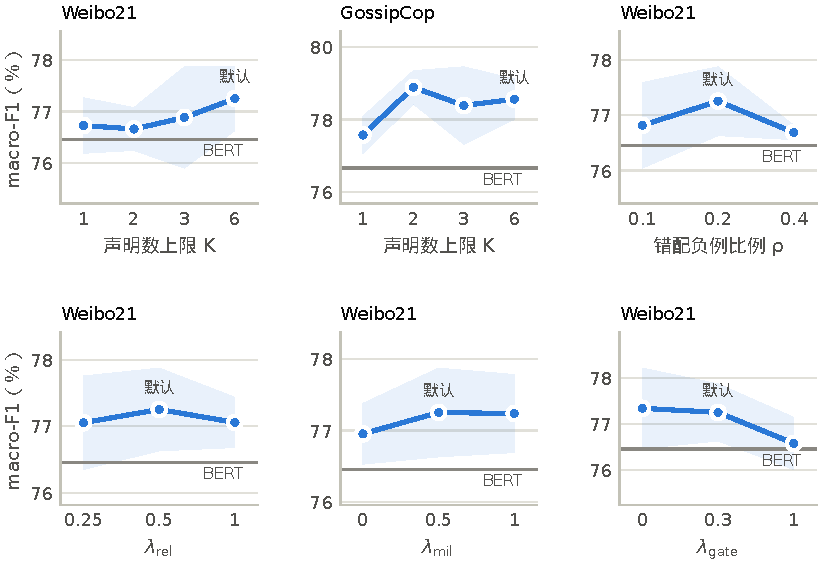
\includegraphics[width=\linewidth]{figures/sensitivity.pdf}
\caption{\method{} 对声明数上限 $K$（两个数据集）以及错配负例比例 $\rho$ 与三个损失权重（Weibo21）的敏感性。每个点为 3 个种子的均值，阴影为标准差；标“默认”的点是正文使用的取值在相同 3 个种子上的结果。灰色横线为 BERT。}\label{fig:sens}
\end{figure}

\section{受控测试集的构建细节}\label{app:perturb}

\paragraph{风格改写}
中文测试集 \cnt{CN/perturb/style_n} 条中有 \cnt{CN/perturb/style_rewritten} 条得到了可用的改写，英文 \cnt{EN/perturb/style_n} 条中为 \cnt{EN/perturb/style_rewritten} 条。被丢弃的主要是改写后长度超过原文 2.5 倍的短消息。作为事实保持程度的粗略代理，我们统计了原文中的数字串在改写后的保留比例：中文为 \pone{CN/fact_preservation/kept_rate}\%，英文为 \pone{EN/fact_preservation/kept_rate}\%。这只是一个代理指标，改写仍可能增删细节，这是 LLM 风格攻击的共同局限\citep{wu2024sheepdog}。

\paragraph{单句事实篡改}
候选为测试集中至少含两句、且存在长度足够的句子的真新闻（中文 \cnt{CN/perturb/tamper_candidates} 条，英文 \cnt{EN/perturb/tamper_candidates} 条）。篡改模型给出的片段必须在句中恰好出现一次，替换后字母与数字内容必须发生变化，且替换不得改变分句结果。最终得到中文 \cnt{CN/perturb/tamper_n} 条、英文 \cnt{EN/perturb/tamper_n} 条，平均每条分别含 \fone{CN/perturb/tamper_mean_sents} 与 \fone{EN/perturb/tamper_mean_sents} 句。按篡改类型的定位结果见表~\ref{tab:loc-type}。

\begin{table}[H]
\centering\small
\caption{按篡改类型划分的定位 Hit@1（\%）。}\label{tab:loc-type}
\fittable{tables/loc_type.tex}
\end{table}

\section{样例}\label{app:cases}

下面两条样例按预先固定的规则选出：篡改测试集中按编号排序、含 3--4 句且不超过 170 个字符的前两条，取随机种子 1 的模型输出，未做任何人工挑选。被篡改的句子与其原句用〔〕标出；表中 $+$ 与 $-$ 分别为 LLM 写出的支持论证与质疑论证。

\noindent\textbf{样例 1}（篡改类型：实体；\method{} 预测 $\hat y=0.00$）\par
{\small\begin{quote}
[1] \textbf{〔被篡改〕}【华为隐形指纹技术正式亮相】\quad\textbf{〔原句〕}【vivo隐形指纹技术正式亮相】\par
[2] 全面屏手机时代即将到来。\par
[3] 如此一来前后指纹已成为过去式，所有手机设计上又将站在同一起跑线了，大家觉得屏幕内指纹解锁帅不帅？秒拍视频\par
\end{quote}}
{\small\begin{tabularx}{\linewidth}{@{}clXccc@{}}
\toprule
句 & 类型 & 声明与两方论证 & $v_k$ & $g_k$ & $p_k$ \\
\midrule
-- & 整体 & \textbf{这条消息整体的可信度}\newline $+$ 全面屏手机的发展趋势确实存在。\newline $-$ 消息中提到的华为隐形指纹技术未得到官方证实。 & 0.74 & 0.23 & 0.00 \\
1 & 事实 & \textbf{华为隐形指纹技术正式亮相}\newline $+$ 华为经常发布新技术，此消息可能为谣言。\newline $-$ 华为官方未发布过此消息。 & 0.59 & 0.62 & 0.01 \\
2 & 观点 & \textbf{全面屏手机时代即将到来}\newline $+$ 手机厂商都在研发全面屏，此说法有一定合理性。\newline $-$ 全面屏技术仍在发展，尚未普及。 & 0.45 & 0.54 & 0.00 \\
\bottomrule
\end{tabularx}}
\par\medskip
\noindent\textbf{样例 2}（篡改类型：实体；\method{} 预测 $\hat y=0.00$）\par
{\small\begin{quote}
[1] 【天津健康码亮码超2100万次集成新功能后将沿用】\par
[2] 很多人关心疫情过后，天津健康码是否还会沿用？\par
[3] 在3月19日召开的新闻发布会上，天津市大数据管理中心主任边柯柯就此回应称，天津健康码将联合津心办一网通办平台，集成更多便民服务应用，继续沿用下去。\par
[4] \textbf{〔被篡改〕}边柯柯介绍说，天津将积极推动电子通行证在互联网+医疗健康相关场景的应用，实现签约预约\quad\textbf{〔原句〕}边柯柯介绍说，天津将积极推动健康码在互联网+医疗健康相关场景的应用，实现签约预约\par
\end{quote}}
{\small\begin{tabularx}{\linewidth}{@{}clXccc@{}}
\toprule
句 & 类型 & 声明与两方论证 & $v_k$ & $g_k$ & $p_k$ \\
\midrule
-- & 整体 & \textbf{这条消息整体的可信度}\newline $+$ 声明直接引用了官方发言，具有较高的可信度。\newline $-$ 消息中提及的具体日期和发言人姓名不明确，且部分内容为预测性意见，缺乏具体细节。 & 0.52 & 0.50 & 0.01 \\
3 & 引述 & \textbf{天津市大数据管理中心主任边柯柯在3月19日的新闻发布会上表示，天津健康码将集成更多便民服务应用，继续沿用下去。}\newline $+$ 该声明直接引用了官方发言，具有较高的可信度。\newline $-$ 新闻发布会的具体日期和发言人姓名未明确提及，可能存在信息不准确的风险。 & 0.23 & 0.82 & 0.01 \\
4 & 观点 & \textbf{天津将积极推动电子通行证在互联网+医疗健康相关场景的应用。}\newline $+$ 这是官方对未来发展的积极展望，符合政策导向。\newline $-$ 该说法是预测性意见，缺乏具体实施细节和时间表，可信度较低。 & 0.64 & 0.89 & 0.03 \\
\bottomrule
\end{tabularx}}
\par\medskip


\section{未使用的数据集}

LIAR-RAW 与 RAWFC 的价值在于为每条声明检索到的原始报道，闭卷条件下只剩一句很短的声明，且 \citet{thibault2025guide} 指出 LIAR 系列中有相当比例的样本本身不可核查；FakeNewsNet 的原始发布不含正文，只有标题与推文编号；SciFact 是需要证据文档的科学声明核查任务。它们与本文的闭卷、纯文本、新闻级检测设定不符，故未使用。
